\documentclass[a4paper]{scrartcl}
\pagestyle{headings}
\usepackage{mdwlist}
\usepackage{polski}
\usepackage[utf8x]{inputenc}
\usepackage{color}
\usepackage{mathtools}
\usepackage{graphicx}
\usepackage[unicode=true]{hyperref}
\usepackage{multirow}
\usepackage[table]{xcolor}
\usepackage{listings}

\lstset{ %
basicstyle=\footnotesize,       % the size of the fonts that are used for the code
numbers=left,                   % where to put the line\dywiz numbers
numberstyle=\footnotesize,      % the size of the fonts that are used for the line\dywiz numbers
stepnumber=2,                   % the step between two line\dywiz numbers. If it's 1, each line 
% will be numbered
numbersep=5pt,                  % how far the line\dywiz numbers are from the code
frame=single,                   % adds a~frame around the code
}

\begin{document}

\sloppy

\newcommand{\ttt}{$T^3\:$}

\title{\ttt - Twórca Tablic Tęczowych}
\subtitle{Równoległe wyznaczanie tęczowych tablic (``rainbow tables'') w~zgadnieniach kryptografii dla haseł zaszyfrowanych algorytmem DES: Scala}
\author{Bartosz Pieńkowski, Barnaba Turek}
\maketitle
\section{Opis}
\ttt to zestaw programów wyznaczających tablice tęczowe i~pozwalających sprawdzić poprawność ich wyznaczenia (przez wyznaczenie funkcji skrótu dla danego ciągu znaków (dalej klucza) i~próbę odwrócenia tego procesu).

\emph{Tablice tęczowe} to sposób przechowywania wcześniej obliczonych danych pozwalających odwracać (analitycznie nieodwracalną) funkcję skrótu\footnote{inaczej kryptograficzną funkcję mieszającą, ang. \emph{hash function}}.
\emph{Tablice tęczowe} pozwalają zmniejszyć wymagania dyskowe (w~stosunku do prostego zapisywania wszystkich par klucz\dywiz f(klucz)) kosztem wymagań obliczeniowych.
Osiągane to jest za pomocą tworzenia tzw. łańcuchów skrótów\footnote{ang. \emph{hash chaining}} i~zapisywaniu tylko pierwszego i~ostatniego elementu łańcucha.

\subsection{Funkcja skrótu}
\ttt wyznacza \emph{tablice tęczowe} dla funkcji skrótu \textbf{md5}.

\section{Użycie}
\subsection{Tworzenie tablic tęczowych}
Program generujący tablice tęczowe nazywa się \emph{t3}.

\subsubsection{Wywołanie programu}
Użytkownik programu t3 podaje trzy argumenty linii poleceń. Pierwszy argument określa długość klucza, dla którego mają być wygenerowane \emph{tablice tęczowe} (od 1 do 8).
Drugi argument określa długość obliczanych łańcuchów.
Trzeci argument określa plik, w~którym mają być zapisane klucze.

\subsubsection{Wyjście programu}
Tablice tęczowe zostaną zapisane w~podanym pliku.
Program tworzy plik, składający się z~wierszy. Każdy wiersz składa się z~początkowego i~końcowego elementu łańcucha skrótów, oddzielnoych spacją.
Łańcuchy są uporządkowane wg. końcowego łańcucha, aby przyspieszyć wyszukiwanie.
Na początku pliku znajduje się nagłówek określający długość łańcuchów, alfabet z~którego są zbudowane i~długość kluczy.

\subsubsection{Przykładowe wywołania}
Wywołanie:
\begin{lstlisting}
  $ t3 2 10
\end{lstlisting}
Wygeneruje tablice tęczowe dla haseł o~dłguości dwóch znaków. Łańcuchy skrótów będą miały długość 10.

Do generowania skrótów służy program \emph{t3-hash}.
\subsubsection{Wywołanie programu}
Użytkownik programu \emph{t3-hash} jako argument podaje klucz (1 do 8 znaków), dla którego ma być wygenerowany skrót.
Następnie program wypisuje skrót na standardowe wyjście.

\subsection{Odwracanie funkcji skrótu}
Do odwracania funkcji skrótu służy program \emph{t3-reverse}.
\subsubsection{Wywołanie programu}
Użytkownik programu \emph{t3-reverse} jako argument podaje wartość funkcji skrótu, dla której znaleziona ma być wartość klucza.

Jako drugi argument należy podać ścieżkę do pliku z~tablicami tęczowymi wygenerowanymi przez \ttt.

Jeżeli program nie znajdzie klucza pasującego do zadanej wartości funkcji skrótu, program zakończy działanie wypisując informację o~niepowodzeniu.

Jeżeli działanie programu zakończy się sukcesem, program wypisze znaleziony klucz. Poprawność znalezionego klucza będzie można sprawdzić korzystając z~programu \emph{t3-hash}.

\subsubsection{pokrycie zbioru kluczy}
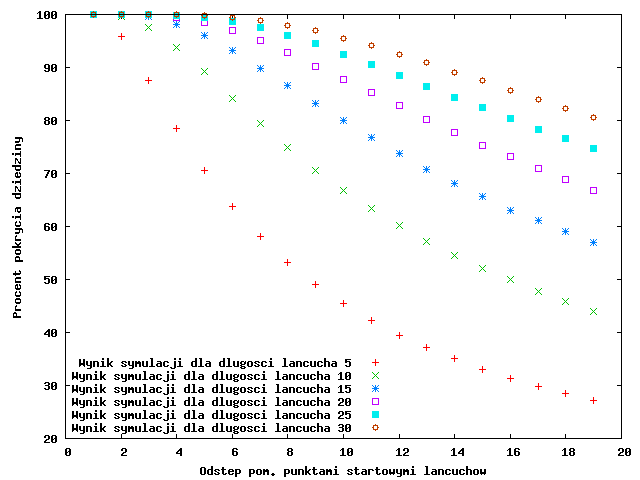
\includegraphics[width=\textwidth]{pokrycie.png}

\section{Implementacja}
\subsection{Rozwiązania}
%Program zostanie wykonany w~języku \textbf{Scala} na platformę \textbf{JVM}.

\subsubsection{Redukcja}
Wynik funkcji MD5 to 16 bajtów.
Możemy to zapisać jako 4 zmienne typu int.

\begin{lstlisting}
    for (int i=0; i<4; i++){
      hash[i] = getInt(MD5Bytes.slice(i*4,(i+1)*4));
      hash[i] = idx ^ (redux_number << (i*4));
    }
\end{lstlisting}

Następnie z~każdej zmiennej tworzymy cztery indeksy do tablicy reprezentującej alfabet.
\newpage
\emph{AlphaLen}\dywiz liczba elementów w~tablicy.

\begin{lstlisting}
  val pwd = Buffer[Int];
  for (int i=0; i<4; i++){
     pwd += (hash[i] % AlphaLen^2) / AlphaLen;
     pwd += (hash[i] % AlphaLen^2) % AlphaLen;
     pwd += ((hash[i] / AlphaLen^2) % AlphaLen^2) / AlphaLen;
     pwd += ((hash[i] / AlphaLen^2) % AlphaLen^2) % AlphaLen;
  }

  //mieszanie w~celu zroznicowania kolejnych redukcji

  if (redux_number > 16)
    pwd = pwd.reverse();
  
  val slice = pwd.slice(0,redux_number%16);
  pwd.trimStart(redux_number);

  if (redux_number > 32)
    pwd = pwd.reverse();
  elseif (redux_number > 48)
    slice = slice.reverse();

  pwd += slice;
\end{lstlisting}

Następnie elementy pwd są mapowane na znaki ze słownika i~żądana liczba elementów z~początku bufora pwd jest zwracana jako nowy klucz.

Tak zaplanowana funkcja redukcji powinna działać dośc dobrze dla alfabetów nie dłuższych niż 84 znaki.

\subsubsection{Generowanie tablic}
Zrównoleglenie wyznaczania tablic tęczowych zostanie osiągnięte za pomocą mechanizmu Aktorów oferowanego przez język \textbf{Scala}.
Mechanizm ten jest zrealizowany na wirtualnej maszynie Javy za pomocą wątków.

Zamierzamy wykorzystać komunikację globalną - jeden wątek będzie zarządzał wszystkimi innymi wątkami.

Naszym zdaniem najlepszą dekompozycją problemu przy tak postawionym zadaniu będzie dekompozycja domenowa, tj. równomierny podział początkowych\footnote{zaczynających łańcuch skrótów} kluczy na wątki.

Klucze będą dzielone na paczki o~określonym, stałym rozmiarze. Na początku aktor zarządzający procesem wyśle wiadomość do każdego aktora\dywiz wykonawcy.
Wiadomość będzie zawierała informacje o~początkowych kluczach, dla których mają zostać wygenerowane łańcuchy.
Wykonawcy po obliczeniu wszystkich kluczy, których obliczenie zostało im zlecone, wyślą do zarządcy wiadomość zawierającą nazwę pliku tymczasowego, w~którym zapisali posortowane łańcuchy.
Zarządca doda nazwę pliku do kolejki (FIFO) plików, które muszą zostać połączone.

Następnie, kiedy cały zadany zakres kluczy zostanie już znaleziony, zostaną utworzeni nowi aktorzy, odpowiedzialni za scalanie plików.
Zarządca wyśle do każdego z~nich wiadomość zawierającą nazwy dwóch pierwszych plików z~kolejki, które należy scalić.
Ponieważ dane w~plikach są posortowane, scalanie będzie się odbywać na zasadzie podobnej do scalania w~algorytmie merge-sort.
Po skończeniu scalania dwóch plików, aktor zapisze scalone dane do trzeciego pliku, usunie dwa pliki wejściowe i~prześle zarządcy wiadomość zawierającą nazwę nowego pliku.
Zarządca odbierze wiadomość i~doda plik do kolejki plików wymagających scalenia.

Kiedy w~kolejce zostanie tylko jeden plik, zarządca doda do pliku niezbędne nagłówki i~program zakończy działanie.

\begin{figure}
\begin{center}
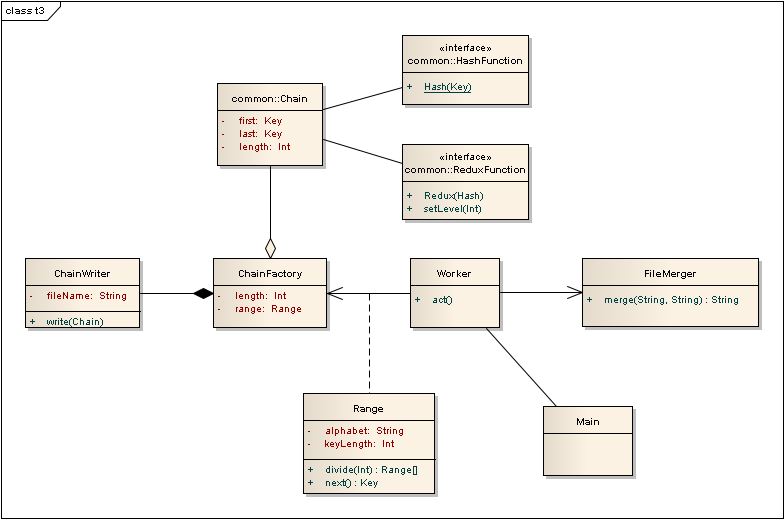
\includegraphics[width=\textwidth]{t3.png}
\end{center}
\caption{diagram klas programu \ttt}
\end{figure}


\subsubsection{Wyszukiwanie}
Program wyszukujący nie będzie podlegał zrównolegleniu, ponieważ jego szybkość będzie w~znacznej mierze ograniczona przez prędkość dowolnego dostępu do dysku.

Na początku program wczyta nagłówek tablicy i~ustawi odpowiednie wartości długości kluczy, do których były przeprowadzane redukcje, długości łańcuchów i~alfabetu.
Program będzie obliczał coraz dłuższe łańcuchy na podstawie klucza(zaczynając od łańcucha jednoelementowego) i~próbował znaleźć łańcuch o~takim samym zakończeniu co obliczone w~tablicach.

Jeżeli wyszukiwanie się nie powiedzie, program wygeneruje dłuższy łańcuch (chyba, że przekroczona zostanie długość łańcucha, dla którego generowana była tablica tęczowa - jeśli tak, program zakończy się niepowodzeniem).

Jeżeli łańcuch znajdujący się w~tablicy zostanie dopasowany do obliczonego łańcucha długości $n$, program wczyta pierwszy element łańcucha i~wygeneruje na jego podstawie łańcuch o~długości $n-m$ (gdzie m to długość łańcuchów, dla których wygenerowana była tablica). Ostatni element tego łańcucha, to szukany klucz.
\begin{figure}
\begin{center}
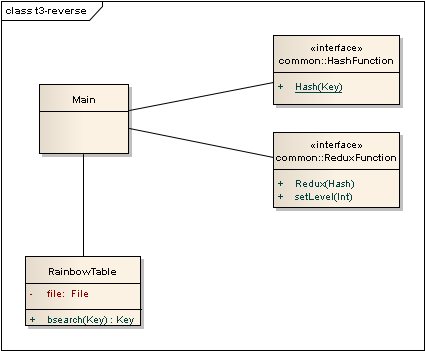
\includegraphics{t3-reverse.png}
\end{center}
\caption{diagram klas programu t3-reverse}
\end{figure}

\begin{figure}
\begin{center}
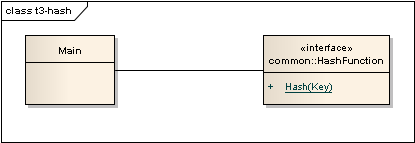
\includegraphics{t3-hash.png}
\end{center}
\caption{diagram klas programu t3-hash}
\end{figure}
\end{document}
